\documentclass{standalone}
\usepackage{xr}
\externaldocument{../Chapter2/intro}
\begin{document}
\subsection{Segmentation}
Once trained, the CNN model was used for the segmentation of the MRI scans of each patient.
Before the segmentation, the scans are pre-processed as previously described.
\\
The segmentation is done slice by slice, for each patient, by using the trained CNN model to obtain the predicted tumor area.
The prediction values range between 0 and 1.
\\
Then, using \textsc{OpenCV}\cite{opencv_library} functions it is possible to obtain a segmented area like the one in Figure \ref{contoured}, where the red contour represents the border of the predicted tumor area.


\begin{figure}[htp]

    \centering
    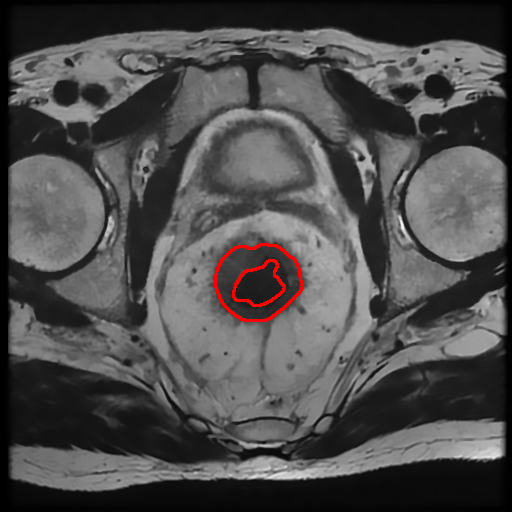
\includegraphics[width=.49\textwidth]{../images/BO56_9_cont.png}
    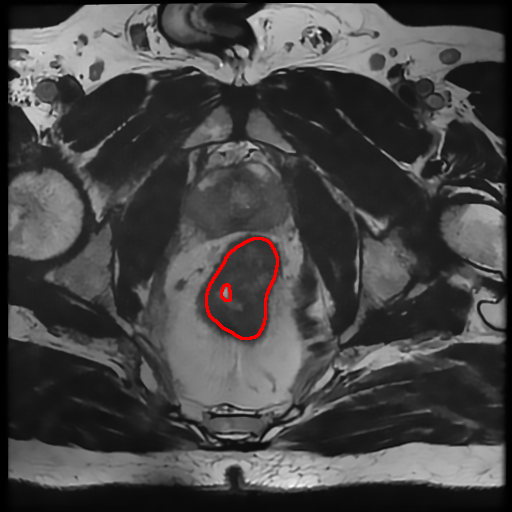
\includegraphics[width=.49\textwidth]{../images/BO85_6_cont.png}
    
    \caption{Images of colorectal cancer with identified tumor areas from two different patients. The red contour represents the border of the predicted tumor area.}
    \label{contoured}
    
    \end{figure}


\end{document}